\documentclass[conference]{IEEEtran}
\IEEEoverridecommandlockouts
\usepackage{cite}
\usepackage{amsmath,amssymb,amsfonts}
\usepackage{algorithmic}
\usepackage{mathpazo}
\usepackage[spanish]{babel}
\usepackage[utf8]{inputenc}
\usepackage{graphicx}
\usepackage{textcomp}
\usepackage{xcolor}
\usepackage{url}
\usepackage{ctable}
\usepackage{float}
\usepackage{amsmath,amssymb,amsfonts}
\usepackage{makecell}
\usepackage{hyperref}
\usepackage{comment}
\usepackage{csquotes}
\hypersetup{
	colorlinks=true,
	linkcolor=blue,
	filecolor=magenta,      
	urlcolor=cyan,
}
\newcommand{\DNoise}{n_d}

\newcommand{\Est}[1]{\hat{#1}}
\newcommand{\Test}[1]{\expandafter\hat#1}


\def\BibTeX{{\rm B\kern-.05em{\sc i\kern-.025em b}\kern-.08em
    T\kern-.1667em\lower.7ex\hbox{E}\kern-.125emX}}

\makeatletter
\newcommand{\linebreakand}{%
  \end{@IEEEauthorhalign}
  \hfill\mbox{}\par
  \mbox{}\hfill\begin{@IEEEauthorhalign}
}
\makeatother
\begin{document}
\title{\bf{El Razonamiento Matemático de modelos Transformer}}
\author{
\IEEEauthorblockN{Jesús A. Torrejón León}
\IEEEauthorblockA{\textit{Universidad Nacional de Ingeniería}\\
Lima, Perú\\
\texttt{jtorrejonl@uni.pe}}
\and
\IEEEauthorblockN{Jordi J. Bardales Rojas}
\IEEEauthorblockA{\textit{Universidad Nacional de Ingeniería}\\
Lima, Perú\\
\texttt{jbardalesr@uni.pe}}
\and
\IEEEauthorblockN{Walter J. Felipe Tolentino}
\IEEEauthorblockA{\textit{Universidad Nacional de Ingeniería}\\
Lima, Perú\\
\texttt{wfelipet@uni.pe}}}
\maketitle

\begin{abstract}

En este trabajo ...
\vspace{0.2cm}

\'Indice de T\'erminos— ...
\end{abstract}

\section{Introducci\'on}
% Presentación del problema general sobre el que versará el trabajo y cómo se
% integra dentro del uso del lenguaje python y sus librerías en el curso.
% - Objetivo del estudio
% - Organización del informe (secciones).
% - Estado del arte
% - Breve mención del aporte que otros artículos científicos han realizado para este problema.
% - Mención de al menos 3 artículos científicos que mencionan el problema y las variantes
% realizadas.
% - Metodología


Las redes neuronales están aún lejos de lograr la robustez y flexibilidad exhibida por humanos al procesar una gran cantidad de diferentes estímulos a la vez, debido a que se encuentran limitadas en su capacidad de generalización y de usar su propia experiencia para manejar con gran precisión entradas no esperadas construidas naturalmente \cite{b3}.

Existen diversas áreas donde resulta un gran reto aplicar modelos inteligentes sin escapar de dichas limitaciones naturales. Una de esas áreas es la \textbf{generalización algebraica}, aquí se forman generalizaciones a partir de experiencias con símbolos, luego se formalizan esas ideas y se explora conceptos de patrones y funciones sobre cualquier clase de objetos y entidades, resultando dominios complejos de manipular y cuyo razonamiento es claramente diferente al tipo de generalizaciones que nos permiten, por ejemplo, traducir una nueva oración del Francés al Inglés \cite{b5, b3}.

El objetivo general de este estudio es superar las limitaciones producidas naturalmente cuando queremos producir razonamiento y generalización algebraica en un modelo Transformer introducido en el artículo  \enquote{\textit{Attention is all you need}} del 2017, véase la referencia \cite{b4}. Para poder medir la capacidad de generalización y razonamiento del modelo primero debemos tener en cuenta la variedad de habilidades cognitivas matemáticas que usan los humanos para superar estás limitaciones, veamos esto considerando el siguiente ejemplo matemático presentado en \cite{b3}. 
\textit{$$\text{¿Cuál es la regla de correspondencia de } g(h(f(x)))$$
$$ \text{donde } f(x)= 2x+3, g(x)=7x-4 \text{ y } h(x)=-5x-8 \text{?}$$}
Dentro de una serie de habilidades matemáticas que el humano realiza para responder a esa pregunta se encuentran: Interpretar los caracteres en entidades (tales como números, operadores aritméticos, variables y las palabras que determinan el contexto de la pregunta), organizar e identificar las funciones en el correcto orden para componerlas, usar reglas aritméticas, almacenar los valores intermedios para la composición y aplicar conocimientos adquiridos sobre transformaciones y axiomas \cite{b3, b2}. Estas reglas de solución pueden ser parte de un algoritmo computacional para resolver únicamente esa clase de problemas, empleando instrucciones pre-programadas y ejecutándolas con buena precisión, sin embargo esto escapa de cualquier tipo de generalización del problema. Además por el amplio tipo de preguntas tales como 
\textit{$$\text{¿Cuánto es f(x) si f(x) = 4x - 1, x = 4 + z \text{ y } z=3?}$$
$$\text{Calcula -666.1234 + 31415.55}$$
$$\text{Resuelve 4x = 20}$$
$$\text{Si tengo 4 manzanas y me como una ¿cuántas quedan?}$$}
Resulta la necesidad de crear un modelo que trate de imitar el razonamiento humano pero sin el uso de algoritmos computacionales pre-programados para cada problema. Lo que se proponer es leer a nivel de carácter sentencias con expresiones matemáticas de un conjunto de datos (con una naturaleza de razonamiento discreto), entrenar y evaluar las expresiones en un modelo capaz de interpretar el contexto para retornar el resultado con buena precisión. Frente a este desafió encontramos tres interesantes trabajos de investigación

En el trabajo \cite{b2} de Artit Wangperawong títulado \enquote{\textit{Attending to Mathematical Language with Transformers}} del 2019 presenta tres modelos Transformer (Básico, Universal y Adaptativo) para leer sentencias con la siguiente estructura $x=85, y = -523, x \times y$, para luego retornar el valor de la operación $-44455$, para esto se ofusca los números, variables y símbolos de la secuencia de entrada a letras. Además se emplea 12 millones de muestras únicas generadas y repartidas aleatoriamente en conjuntos de entrenamiento y prueba con la proporción de 9 a 1. Por otro lado en el estudio de 
Lukasz Kaiser y Ilya Sutskever \cite{b5} se modelan operaciones de adición y multiplicación binaria, y está restringido a enteros con el mismo número de dígitos y no involucra variables simbólicas o expresiones que determinen el contexto de la operación. Finalmente el trabajo que hemos tomado como referencia principal, cuyos autores son Saxton, Kohli, Grefenstette y Hill, títulado \enquote{\textit{Analysing Mathematical Reasoning Abilities of Neural Models}} \cite{b3} del 2019, muestra modelos Transformer que permiten generalizar nociones algebraicas, para esto se parte de un conjunto de datos de matemática básica (extraído de un plan de estudio escolar de los Estados Unidos) como las operaciones aritméticas, ecuaciones, funciones, polinomios, entre otras, para luego realizar pruebas de interpolación y extrapolación a partir de un conjunto de datos especial que sometan al modelo a generalizar nociones aprendidas, ya sea evaluar funciones en dominios no entrenados o combinar conocimientos de funciones, ecuaciones, derivadas, entre otros, por ejemplo hallar la derivada de la composición de dos funciones, resultando aprender la regla de la cadena.

El presente artículo abarca el \textbf{diseño} de los Transformer, modelo cuyo concepto fundamental son las capas de atención, para afrontar las límitaciones de modelos recurrentes como el LSTM, GRU, entre otros. Además se implementa en Python las clases necesarias para construir los Transformer, para que luego sean entrenados y puestos a prueba. Finalmente discutiremos los resultados y compararemos con los estudios de referencia para luego sacar nuestras propias conclusiones y dar alternativas de trabajos a futuro.


\section{Diseño}
% Descripción de los objetos, funciones y técnicas a utilizar
Una mejora de los modelos Seq2Seq (Sequence to Sequence) con redes neuronales recurrentes consiste en introducir mecanismos de atención entre las capas encoder y decoder, para producir un contexto más solido, representado por el vector $c_t$ de la figura \ref{fig::seq2seq-attention}, de lo contrario el decoder generará la secuencia de salida a partir de únicamente el vector del estado oculto de transición (también llamado vector de pensamiento $h_t$), este vector acumula celda por celda toda la información de la secuencia de entrada, por lo que \enquote{recordará} mejor los valores ocultos de las últimas celdas que de las iniciales, lo que puede originar mala atención, cuellos de botella y sobreajuste. Para afrontar este problema se mejoran los modelos agregando mecanismos de atención, de esta manera el decoder puede consultar en cualquier paso de tiempo la información que hubo en cualquiera de las celdas del encoder \cite{b1}. 

\begin{figure}[ht]
\centering
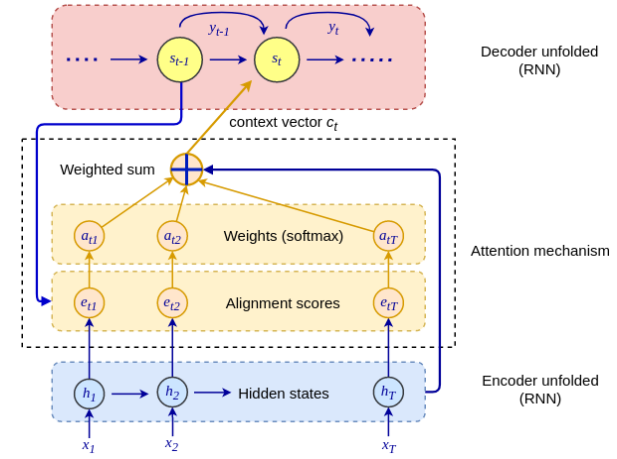
\includegraphics[width=0.47\textwidth]{PC5/seq2seq-attention.png}
\caption{Mecánismo de atención Bahdanau o Additive en un modelo estándar Seq2Seq \cite{b1}.}
\label{fig::seq2seq-attention}
\end{figure}

Sin embargo al seguir trabajando en el contexto de Redes Neuronales Recurrentes se suele generar una secuencia de estados ocultos $h_t$ a partir del estado oculto anterior $h_{t-1}$ y la entrada en la posición $t$, esta naturaleza secuencial de procesamiento impide la paralelización, lo que se vuelve crítico a mayor longitudes de secuencia, ya que las restricciones de memoria limitan el procesamiento por lotes. En \cite{b4} se propone la creación de un modelo llamado \textbf{Transformer} que evita la recurrencia y en su lugar confiando enteramente en mecanismos de atención para generar dependencias globales entre la entrada y la salida, además permitiendo la paralelización en sus capas de atención. 



\subsection{Mecánismos de Atención}
Los mecanismos de atención son el eje fundamental del desarrollo del presente trabajo, conforman la base de los Transformer.

Una función de atención puede ser descrita como un mapeo de una consulta (cuyo conjunto de consultas se empaqueta en una matriz Q y en la práctica se calcula la función de atención sobre esta matriz Q) y un conjunto de pares clave-valor (empaquetados en matrices K y V) a una salida. 

Existen varios mecanismos de atención que se muestra en la literatura, sin embargo para entender los Transformer nos enfocaremos en los más sofisticados para modelos que a priori son complejos de modelar \cite{b4}.

\subsubsection{Scaled Dot-Product}
La entrada consiste de vectores consultas $Q$ y vectores claves $K$ de dimensión $d_k$, y valores $V$ de dimensión $d_v$. Luego se sigue una serie de operaciones, resultando la salida como una suma ponderada de $V$.

\begin{figure}[ht]
\centering
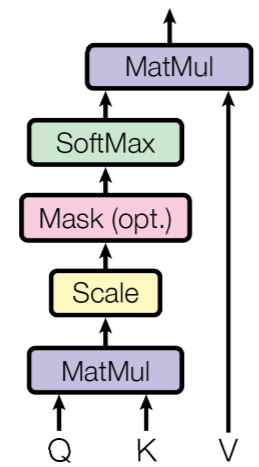
\includegraphics[width=0.15\textwidth]{PC5/scale-dot-product.png}
\caption{Flujo del mecanismo de atención Scaled Dot-Product \cite{b4}}
\label{fig::scale-dot-product}
\end{figure}

De acuerdo a la figura \ref{fig::scale-dot-product} el flujo comienza calculando el producto punto de las consultas y las claves, luego escala por $1/\sqrt{d_k}$ y aplica una función softmax para obtener los pesos necesarios para realizar la suma ponderada sobre el vector de valores $V$. Este procedimiento se representa en la siguiente ecuación

$$
\text{Attention}(Q,K,V)= \text{softmax}(\dfrac{QK^T}{\sqrt{d_k}})
$$

De acuerdo a la literatura existen dos funciones de atención muy usadas: Additive Attention, también conocida como Bahdanau Attention, y Dot-Attention (Sin el escalado). Ambas ayudan a solucionar el problema de cuello de botella que se origina entre la transferencia de información entre el encoder y decoder. La primera consiste fundamentalmente en agregar más parametros entrenables a un modelo sequence to sequence con estados ocultos en el contexto de las Redes Neuronales Recurrentes, aumentando la complejidad de cálculo especialmente cuando se trabaja con una gran cantidad de datos de entrenamiento. Aunque ambas tienen una similar complejidad teórica, Dot-Product attention es más rápida y efeciente en el uso del espacio de memoria, puesto que se puede implementar usando técnicas avanzadas y eficientes de multiplicación matricial, sin embargo para pequeñas dimensiones $d_k$ Additive Attention presenta mejores resultado que el mecanismo Dot Attention, y para grandes dimensiones (nuestro interés en particular) los productos punto crecen en magnitud, empujando a la función softmax dentro regiones donde hay gradiente extremadamente pequeños. Para contrarestar este efecto se escala el producto punto por $1/\sqrt{d_k}$, resultando el mecanismo de atención Scaled Dot-Product.

\subsubsection{Multi-Head}
Se trata se mejorar la función de atención al realizar procesamiento paralelo, veasé la figura \ref{fig::multi-head-attention}.

\begin{align*}
\text{MultiHead}(Q,K,V) &=\text{Concat}(\text{head}_1,\ldots,\text{head}_h)W^0, \\
\text{ donde } \text{head}_i &=\text{Attention}(QW^Q_i,KW^Q_i,VW^Q_i)
\end{align*}


\begin{figure}[ht]
\centering
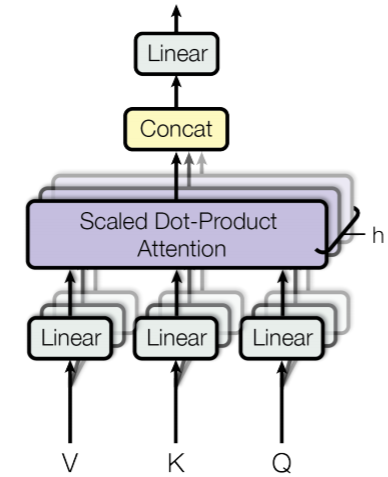
\includegraphics[width=0.3\textwidth]{PC5/multi-head-attention.png}
\caption{Flujo del mecanismo de atención Head-Attention \cite{b4}.}
\label{fig::multi-head-attention}
\end{figure}


\subsection{Transformer}
Consta de una capa Encoder y otra Decoder. 

El Encoder está compuesto por una pila de 6 capas idénticas. Cada capa tiene dos subcapas. El primero es un mecanismo de atención  Multi Head-Attention,  y el segundo es una red de feed forward simple completamente conectada. Además se insertan capas de normalización.

El Decoder también está compuesto por una pila de 6 capas idénticas. Además de las dos subcapas en cada capa del Encoder, el Decoder inserta una tercera subcapa, que realiza una atención Multi Head-Attention sobre la salida de la pila del encoder. De manera similar al encoder, empleamos conexiones residuales alrededor de cada una de las subcapas, seguidas de la normalización de la capa.

La implementación oficial del Transformer se encuentra en el repositorio del paper \enquote{Attention is all you need}.

\begin{figure}[ht]
\centering
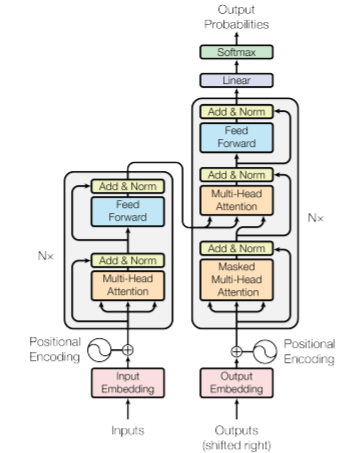
\includegraphics[width=0.4\textwidth]{PC5/transformer-archi.png}
\caption{Arquitectura de un transformer \cite{b4}.}
\label{fig::transformer-archi}
\end{figure}

\subsection{Conjunto de datos}

El dataset utilizado fue creado por los autores del artículo \cite{b7}.

Este posee una estructura modular cuya unidad más básica son las tareas de un mismo tipo y de un mismo nivel de dificultad. Estos archivos de entrenamiento asu vez pertenecen a un área de las matemáticas. Cada una de las áreas se detallara a continuación:

\subsubsection{Algebra}

Algunas de las tareas en esta area incluyen:

  • linear\_1d resolver una ecuacion lineal de una sola variable.
  
  • linear\_2d resolver ecuaciones de dos variables simulaneo.
  
  • polynomial\_roots encuentra las raíces de un determinado polinomio o factoricelo.
  
  • sequence next term Elija una correcta continuación de la secuencia numérica.
  
  • sequence nth term Determine el enésimo elemento de una secuencia dados únicamente los primeros términos.
  

La extrapolación en esta área podrá ser evaluada con las siguientes tareas:

  • polynomial\_roots\_big los coeficientes de los polinomios así como su grado es mayor a los vistos durante el entrenamiento.



\subsubsection{Arithmetica}
  
  • add\_or\_sub suma o resta de un par de números enteros enunciados de distintas maneras.
  
  • add\_or\_sub\_in\_base similar a la anterior con la particularidad de que la base sobre la que se efectúa la suma o resta se encuentra entre 2 y 16.
  
  • add\_sub\_multiple Suma y resta de distintos números. 
  
  • div division de numeros enteros donde la respuesta se encuentra expresada en una fracción irreductible.
  
  • mixed operaciones mixtas involucrando las 4 operaciones básicas así como agrupación por paréntesis.
  
  • mul multiplicación tanto de números enteros como de números decimales.
  
  • nearest\_integer\_root calcular el número más cercano a la raíz enésima de otro numero.
  
  • simplify\_surd Simplificar una expresión que contiene raices cuadradas. 

    
Para evaluar la capacidad de extrapolación en el modelo se incluyen las siguientes tareas:


• add\_or\_sub\_big: suma o resta de números mucho mayores a los vistos en el entrenamiento.

• add\_sub\_multiple: Múltiples sumas con más términos que los vistos en el módulo de entrenamiento.




Para manejar estos datos que se encuentran en formato txt utilizaremos un módulo denominado math\_dataset, este módulo nos permite cargar las partes necesarias del dataset utilizando por debajo una estructura basada en un dataframe de la librería pandas.
Esto nos facilita por ejemplo el tener que cargar una sola de las tareas pertenecientes al dataset y utilizar datalloaders de modo que se obtenga un mayor grado de paralelismo


\begin{figure}[h]
\centering
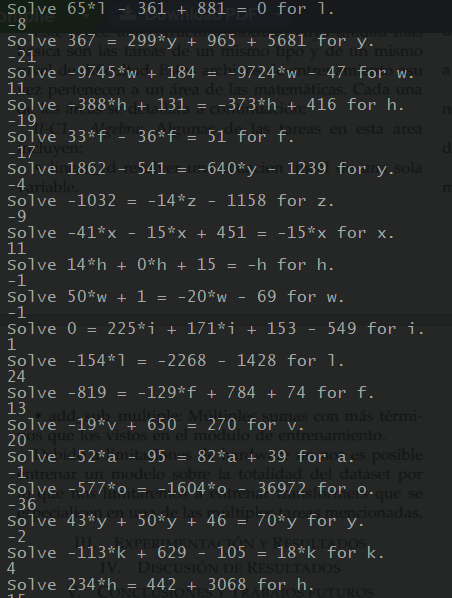
\includegraphics[width=0.4\textwidth]{PC5/linear.png}
\caption{Ejemplos de problemas que podemos encontrar en algebra\_\_linear\_1d nivel medio }
\label{fig::scale-dot-product}
\end{figure}

Debido a limitaciones de hardware no nos es posible entrenar un modelo sobre la totalidad del dataset por lo que nos limitaremos a entrenar transformers que se especialicen en una de las múltiples tareas mencionadas.


\section{Experimentación y Resultados}

\section{Discusión de Resultados}

\section{Conclusiones y Trabajos futuros}

\begin{thebibliography}{00}

\bibitem{b1} Vasilev Ivan. Advanced Deep Learning with Python:  Design and Implement Advanced Next-Generation AI Solutions using TensorFlow and Pytorch.

\bibitem{b2} Wangperawong Artit (2019). Attending to Mathematical Language with Transformers.

\bibitem{b3} Saxton David, Grefenstette, Hill Felix, Kohli Pushment (2019). Analysing Mathematical Reasoning Abilities of Neural Models.

\bibitem{b4} Ashish Vaswani, Noam Shazzer, Niki Parmar, Jakob Uszkoreit, Llion Jones, Aidan Gomez, Lukasz Kaiser, Illia Polosukhin (2017). Attention Is All You Need.

\bibitem{b5} Paying Attention to Algebraic Reasoning. Support Document for Paying Attention to Mathematics Education.

% \bibitem{b6} Lukasz Kaiser, Ilya Sutskever

\bibitem{b7}Saxton, David and Grefenstette, Edward and Hill, Felix and Kohli, Pushmeet (2019). Analysing mathematical reasoning abilities of neural models.

\end{thebibliography}
\end{document}
